%%%%%%%%%%%%%%% Updated by MR March 2007 %%%%%%%%%%%%%%%%
\documentclass[12pt]{beamer}
\usetheme{Boadilla}

\newcommand{\al}{$<$}
\newcommand{\ar}{$>$}

\usepackage{graphicx}
\usepackage{wrapfig}
\graphicspath{ {./graphics/} }

\usepackage{minted}
%\usemintedstyle{colorful}
\setmintedinline{breaklines}

\newcommand{\textinline}{\mintinline{text}}
\newcommand{\cinline}{\mintinline{CGatwick}}
\newcommand{\camlinline}{\mintinline{OCaml}}

\title{Compiling OCaml to WebAssembly}
\author{Paul Durbaba}
\date{10 February 2020}

\begin{document}
	\begin{frame}
		\titlepage
	\end{frame}

	\begin{frame}
		\frametitle{Project Idea}
		\begin{itemize}
			\item Compile OCaml to WebAssembly
			\item WebAssembly: Binary Instruction format for the web
		\end{itemize}
		\begin{center}
			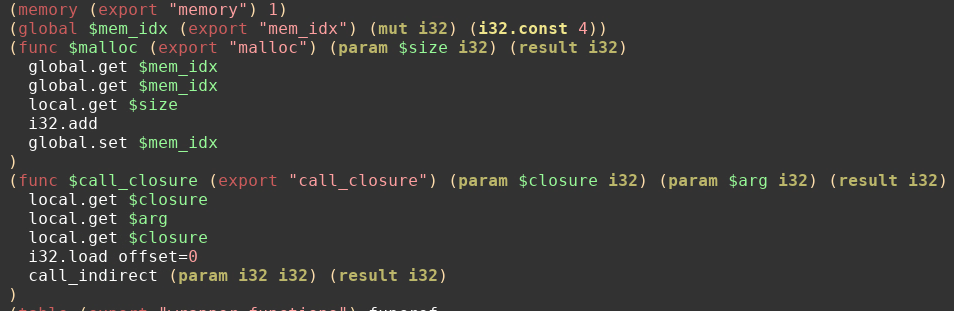
\includegraphics[width=0.8\linewidth]{basic-runtime}
		\end{center}
	\end{frame}

	\begin{frame}
		\frametitle{What I've Achieved}
		\begin{columns}
			\column{0.6\linewidth}
			\begin{itemize}
				\item Type checker (1206 loc) implements Hindley-Milner type inference
				\item Closure conversion (247 loc) gives us top level functions
				\item IR Transformation (1029 loc) designed to target WebAssembly
				\item Code Generation (423 loc) outputs WebAssembly
			\end{itemize}
			
			\column{0.4\linewidth}
			\begin{center}
				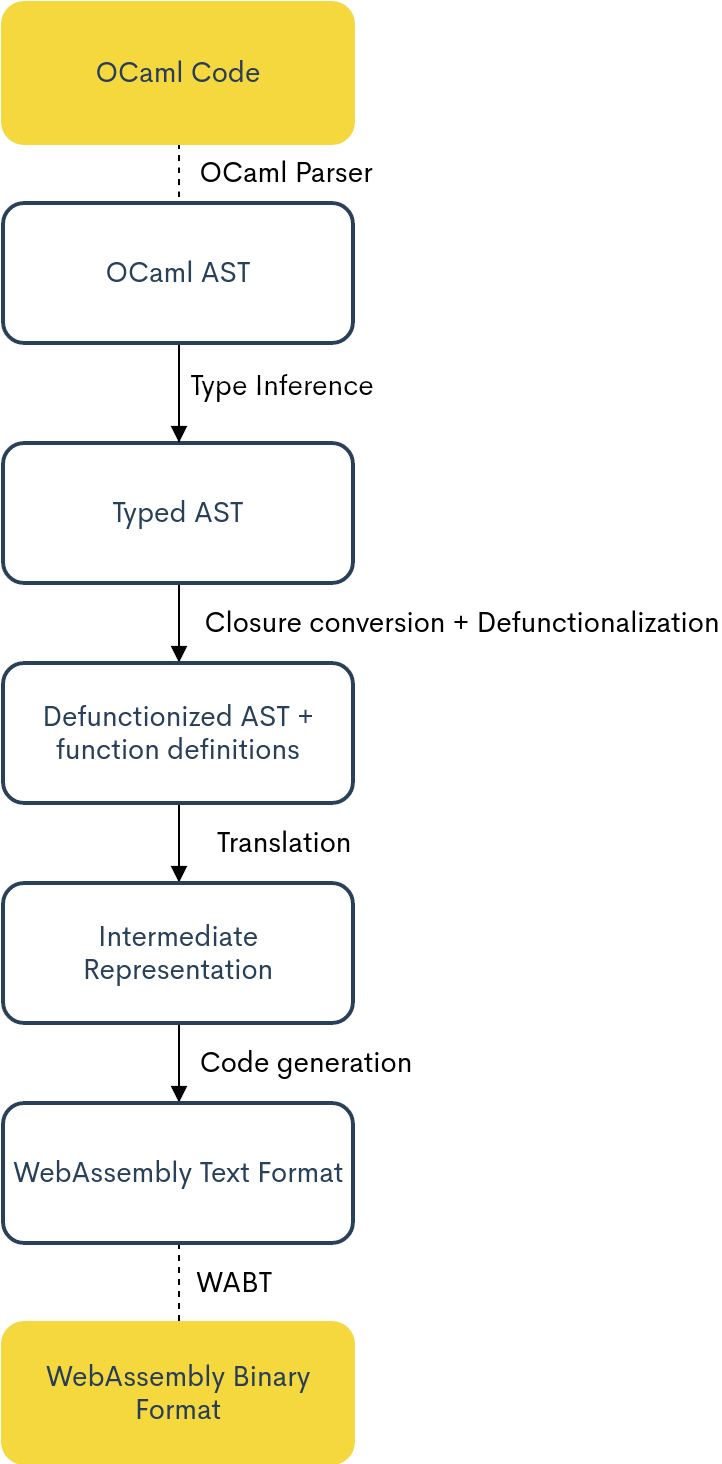
\includegraphics[width=0.55\linewidth]{otwa-diagram}
			\end{center}
		\end{columns}
	\end{frame}

	\begin{frame}[fragile]
		\frametitle{Testing}
		\begin{columns}
			\column{0.6\linewidth}
			\begin{itemize}
				\item End-to-end tester compiles samples and checks their globals computed at runtime
			\end{itemize}
			\column{0.4\linewidth}
			\begin{center}
				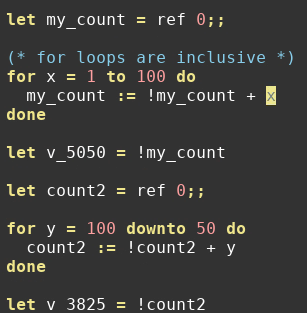
\includegraphics[width=0.55\linewidth]{for-sample}
			\end{center}
			
		\end{columns}
		\begin{center}
			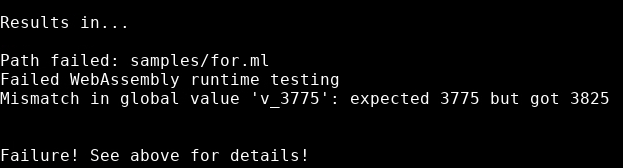
\includegraphics[width=0.6\linewidth]{e2e-output}
		\end{center}
	\end{frame}

	\begin{frame}
		\frametitle{What's Next}
		\begin{columns}
			\column{0.6\linewidth}
			\begin{itemize}
				\item Evaluation benchmarks
				\item Negative tests and error messages
				\item Optimisations (new IR is no longer stack based)
				\item Strings, records, more syntax support
				\item Garbage collection?
				\item Exceptions?
			\end{itemize}
			\column{0.4\linewidth}
			\begin{center}
				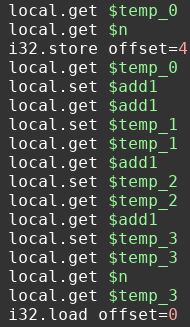
\includegraphics[width=0.55\linewidth]{get-set}
			\end{center}
		    temp\_0 = add1 = temp\_1 = temp\_2 = temp\_3
		\end{columns}
		
	\end{frame}
	
\end{document}
